\chapter{Zielsetzung}
\label{cha:zielsetzung}
In diesem Versuch soll die effektive Masse von Leitungselektronen von n-dotierten Galliumarsenid anhand von Faradayrotation bestimmt werden.

\chapter{Theorie}
\label{cha:Theorie}
Die benötigten theoretischen Grundlagen wie die Bandstruktur der Halbleiter, das Konzept der effektiven Masse und die Faraday-Rotation werden im folgenden Kapitel präsentiert.
\section{Die Bandstruktur eines Halbleiters}
Das Modell der Bandstruktur beschreibt die Überlagerung diskreter Energieniveaus der Elektronen in einem Kristall, hervorgerufen durch
ein gitterperiodisches Potential. Diese Überlagerung verursacht die Entstehung von Energiebändern und Bandlücken. Das Valenzband ist jenes, in dem Elektronen gebunden existieren,
während jene im Leitungsband als delokalisiert angenommen werden können. Ob und unter welchen Bedingungen Elektronen im Leitungsband existieren können,
bestimmen die Eigenschaften eines Materials.\\
Kristalle, dessen Bandlücke zwischen dem Valenz- und Leitungsband größer als $\qty{3}{\electronvolt}$ \cite{bandluecke} ist, sind Isolatoren. Elektronen aus dem Valenzband können unter keinen Bedingungen in 
das Leitungsband angeregt werden. Für Metalle überlappen sich beide Bänder, wodurch das Material dauerhaft leitend wird. Falls eine Bandlücke zwischen 
Leitungs- und Valenzband existiert, welche klein genug ist ($E_{\text{gap}}=\qtyrange{0}{3}{\electronvolt}$)\cite{bandluecke} um durch eine Anregung (z.B thermisch) überwunden zu werden, handelt es sich um einem Halbleiter. 
Hier kann bereits eine Anregung über thermische Strahlung reichen, also einer Umegbungstemperatur von über $\qty{0}{\kelvin}$.
Hierbei wird zwischen direkten und indirekten Halbleitern, bei denen entweder eine energetische Anregung oder eine zusätliche Anregung über Phononen nötig ist, unterschieden. Bei dem ersten Fall liegen Maximum und
Minimum des Valenz- und Leitungsband im E-$\vec{k}$-Raum übereinander. Bei dem zweiten ist das Leitungsband um einen $\vec{k}$-Vektor verschoben, sodass Phononen im Prozess beteiligt sein müssen.
Eine schematische Darstellung der Bandstrukturen von Isolatoren, Metallen und Halbleitern ist in \autoref{fig:Bandstruktur} dargestellt.
\begin{figure}
    \centering
    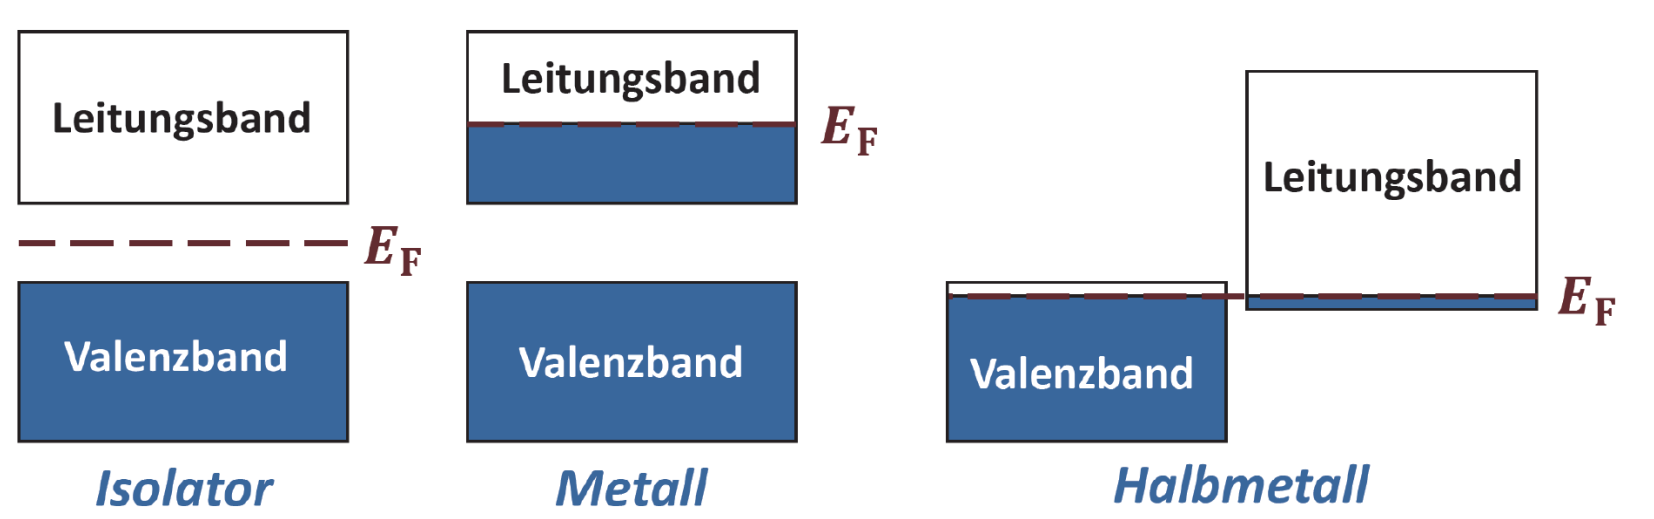
\includegraphics[width = \textwidth]{content/V46_pictures/Bandluecke.png}
    \caption{Schematische Darstellung der Bandstruktur von Isolatoren (links), Metallen (mitte) und Halbleitern (rechts). $E_F$ bezeichnet hier die Fermienergie. \cite{grossmarx}}
    \label{fig:Bandstruktur}
\end{figure}
\\Die Leitfähigkeit eines Halbleiters kann durch eine Dotierung, der Einbringung eines Fremdatoms manipuliert werden. Bei den Atomen wird zwischen Donatoren (bei einer n-Dotierung) und
Akzeptoren (bei einer p-Dortierung) unterschieden.\\
Ein Donator gehört einer höheren Ordnungsgruppe als die Kristallatome, wodurch das überschüssige Elektron des Fremdatoms nur leichte Kräfte 
erfährt und als delokalisiert betrachtet werden kann. Dadurch reichen bereits kleine Energien aus, um das Material leitend zu machen.
Akzeptoren gehören einer niedrigeren Ordnungsgruppe an als die Atome des Kristalls, wodurch ein Überschuss an positiver Ladung folgt.\\
Einer der in diesem Experiment untersuchten Kristalle ist n-dotiertes Galliumarsenid (GaAs), welches ein direkter Halbleiter ist. Galliumarsenid hat eine Bandlücke von $E_{\text{gap, GaAs}} = \qty{1,42}{\electronvolt}$,
wodurch es bei Raumtemperatur nur leicht leitend ist. Dieser Effekt wird durch die Dotierung verstärkt.

\section{Effektive Masse}
Dadurch, dass auf die Elektronen in einem Kristall ein gitterperiodisches Potential wirkt, müssen diese Effekte auf die Bewegung des Elektrons bei der Beschreibung
dessen berücksichtigt werden. Allerdings da das Potential periodisch ist, lässt sich der Effekt mithilfe dem Konzept der effektiven Masse kompensieren, wodurch es möglich ist
das Elektron in harmonischer Näherung frei zu beschreiben. Die Bandstruktur im E-$\vec{k}$-Raum eines Halbleiters ist in \autoref{fig:bandluecke} gezeigt. 
\begin{figure}
    \centering
    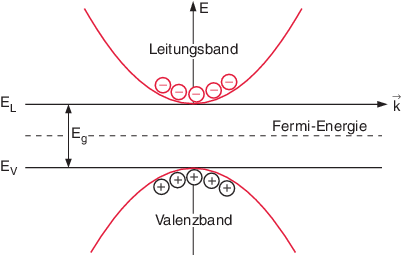
\includegraphics[width = 0.8\textwidth]{content/V46_pictures/Bandstruktur.png}
    \caption{Schematische Darstellung der Bandstruktur von direkten Halbleitern \cite{Demtröder2016}.}
    \label{fig:bandluecke}
\end{figure}
Da diese eine näherungsweise parabolische Form hat, kann man die Energie des Leitungsbandes zunächst mithilfe einer Taylorentwicklung zweiter Ordnung abgeschätzen:
\begin{equation*}
    \mathcal{T}_{(E(\mathbf{k}))} = E(0) + \frac{1}{2}\sum_{\symup{i}=1}^{3}\left(\frac{\partial E^2}{\partial k_{\symup{i}^2}}|_{k=0}\right) k_{\symup{i}}^2 + \mathcal{O}(E(\mathbf{k})^3)
\end{equation*}
Durch einen Vergleich mit $E=\frac{\hbar k^2}{2m}$ lässt sich der Term so umformulieren, dass die sich ergebende Variable die Einheit einer Masse besitzt. Die effektive Masse wird folgend als
\begin{equation*}
    m_{\symup{i}}^{*}=\frac{\hbar^2}{\left(\frac{\partial E^2}{\partial k_{\symup{i}^2}}|_{k=0}\right)}
\end{equation*}
definiert. Die effektive Masse ist durch das dreidimensionale Potential eines Kristalls eine Größe mit Tensoreigenschaften. Bei Kristallen hoher Raumsymmetrie, ist der Tensorcharakter der effektiven Masse
allerdings vernachlässigbar und lässt sich als Skalar beschreiben. Dies ist bei Galliumarsenid der Fall.

\section{Faraday-Rotation}

Eine linear polatisierte Welle besteht aus der Superposition zwei entgegengesetzt zirkular polarisierter Wellen. Durch unterschiedliche Phasengeschwindigkeiten der zirkular polarisierten Wellen
kann es bei der Propagation durch in ein optisches aktiven Medium zu einer Drehung der Polarisationsebene des linear polarisierten Lichts kommen. Dieser Effekt nennt sich zirkulare Doppelbrechung.\\
In optisch inaktiven Medien, wie Galliumarsenid, tritt dieser Effekt unter normalen Umständen nicht auf. Er kann allerdings durch Ausrichtung eines Magnetfeldes parallel zu Ausbreitungsrichtung des 
linear polatisierten Lichts erzwungen werden. Die zirkulare Doppelbrechung in optisch inaktiven Medien durch Einbringung eines Magnetfeldes nennt sich Faraday-Rotation und ist schematisch in \autoref{fig:Faraday} gezeigt.
\begin{figure}
    \centering
    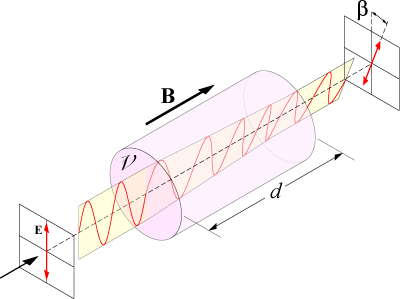
\includegraphics[width = 0.5\textwidth]{content/V46_pictures/Faraday.png}
    \caption{Darstellung der Drehung der Polarisationsebenen einer linear polarisierten Wellen, hervorgerufen durch die Faraday-Rotation \cite{wiki_Fara}}
    \label{fig:Faraday}
\end{figure}
\\Der Drehwinkel, um den die Polarisationsebene der Welle beim Eintritt in das Medium rotiert wird, ist durch
\begin{equation}
    \label{eq:theta}
    \theta = \frac{L\omega}{2}\left(\frac{1}{v_{\text{ph, r}}} - \frac{1}{v_{\text{ph, l}}}\right) = \frac{L\omega}{2c}\left(n_{\text{r}} - n_{\text{l}}\right)
\end{equation}
gegeben. Der Unterschied der Brechungsindize der rechtszirkular polarisierten Welle $n_r$ und linkszirkular polarisierten Welle $n_l$ bestimmt also maßgeblich die Rotation. Ein weiterer
Faktor ist die durchlaufene Strecke im Medium $L$ und die Kreisfrequenz $\omega$. Die Faraday-Rotation ensteht durch magnetisch induzierte elektrische Dipolmomente innerhalb des Kristalle, wodurch eine makroskopische
Polarisation $\vec{P}$ des Stoffs entsteht.\\
Die Suszeptibilität, welche in direkten Zusammenhang mit der Phasengeschwindigkeit der zirkularen Wellen steht, ist von dem angelegten Magnetfeld abhängig über
\begin{equation}
    \chi_\text{xy} = \frac{Ne_0^3\omega B}{\varepsilon_0\left(\left(-m\omega^2+K\right)^2-\left(e_0\omega B\right)^2\right)},
    \label{eq:Suszeptibilitaet_Faraday}
\end{equation}
wobei $\chi_\text{xy}$ die Einträge des Suszeptibilitätstensor sind.\\
Mithilfe von 
\begin{align}
    n_r &= \sqrt{1+\chi_\text{xx}+\chi_\text{xy}} \\
     \text{und } n_l &= \sqrt{1+\chi_\text{xx}-\chi_\text{xy}}
\end{align}
sowie \autoref{eq:Suszeptibilitaet_Faraday} kann \autoref{eq:theta} angenähert werden mit 
\begin{align}
    \theta &\approx \frac{L\omega}{2cn}\chi_{\text{xy}} \label{eq:theta_rl_chi} \\
    &= \frac{e_0^3\omega^2 NBL} {2\varepsilon_0 cm^2\left(\left(\omega_0^2-\omega^2\right)^2-\left(\omega \cdot \omega_\text{c}\right)^2\right)n},
\end{align}
wobei $\omega_0 = \sqrt{\frac{K}{m}}$ die Resonanzfrequenz, $\omega_\text{c} = \frac{e_0B}{m}$ als Zyklotronfrequenz und $m$ die Masse ist. Die Mess- und Resonanzfrequenz
liegt bei Galliumarsenid im Infrarotbereich, wodurch $\left(\omega_0^2 - \omega^2\right)^2 \gg \omega^2\omega_c^2$ gilt, kann der Drehwinkel in Abhängigkeit der Wellenlänge
$\lambda$ der Welle weiter genähert werden:
\begin{equation}
    \theta \approx \frac{e_0^3 NBL 2 \pi^2 c}{\varepsilon_0 m^2 \lambda^2 \omega_0^4 n}.
\end{equation}
Für $\omega_0 \rightarrow 0$ und der effektiven Masse folgt schließlich für die Rotation der Polarisationsebene pro Einheitslänge
\begin{equation}
    \label{eqn:t_frei}
    \theta_\text{frei} \approx \frac{e_0^3 N B}{8\symup{\pi}^2 \varepsilon_0 c^3 (m^*)^2 n} \cdot \lambda^2.
\end{equation}
